\iftestbuild % TEST-ONLY-BEGIN
\setcounter{section}{2}\setcounter{theorem}{38}
\fi % TEST-ONLY-END
% Source: book pp. 319--325 (PDF 333--339).
\section{Consequences of Generalized Eigenspace Decomposition}

\subsection{Square Roots of Operators}

Recall that a square root of an operator $T\in\Lin(V)$ is an operator
$R\in\Lin(V)$ such that $R^2=T$ (see \ref{ax:7.36}). Every complex number has a
square root, but not every operator on a complex vector space has a square
root. For example, the operator on $\C^3$ defined by
$T(z_1,z_2,z_3)=(z_2,z_3,0)$ does not have a square root, as you are asked to
show in Exercise~1. The noninvertibility of that operator is no accident, as we
will soon see. We begin by showing that the identity plus any nilpotent
operator has a square root.

\begin{result}[Identity plus nilpotent has a square root]\label{ax:8.39}
Suppose $T\in\Lin(V)$ is nilpotent. Then $I+T$ has a square root.
\end{result}

\begin{proof}
Consider the Taylor series for the function
$\sqrt{1+x}$:\refstepcounter{theorem}\label{ax:8.40}
\[ \sqrt{1+x} = 1 + a_1x + a_2x^2 + \cdots. \tag{\thetheorem} \]

\marginnote{Because $a_1=1/2$, the formula above implies that
$1+x/2$ is a good estimate for $\sqrt{1+x}$ when $x$ is small.}%
We do not find an explicit formula for the coefficients or worry about whether
the infinite sum converges because we use this equation only as motivation.

Because $T$ is nilpotent, $T^m=0$ for some positive integer $m$. In
\ref{ax:8.40}, suppose we replace $x$ with $T$ and $1$ with $I$. Then the
infinite sum on the right side becomes a finite sum (because $T^k=0$ for all
$k\ge m$). Thus we guess that there is a square root of $I+T$ of the form
\[ I + a_1T + a_2T^2 + \cdots + a_{m-1}T^{m-1}. \]
Having made this guess, we can try to choose $a_1,a_2,\dots,a_{m-1}$ such that
the operator above has its square equal to $I+T$. Now
\begin{align*}
&(I + a_1T + a_2T^2 + a_3T^3 + \cdots + a_{m-1}T^{m-1})^2\\
&\quad= I + 2a_1T + (2a_2+a_1^2)T^2 + (2a_3+2a_1a_2)T^3 + \cdots\\
&\qquad+ (2a_{m-1} + \text{terms involving } a_1,\dots,a_{m-2})T^{m-1}.
\end{align*}
We want the right side of the equation above to equal $I+T$. Hence choose $a_1$
such that $2a_1=1$ (thus $a_1=1/2$). Next, choose $a_2$ such that
$2a_2+a_1^2=0$ (thus $a_2=-1/8$). Then choose $a_3$ such that the coefficient
of $T^3$ on the right side of the equation above equals $0$ (thus
$a_3=1/16$). Continue in this fashion for each $k=4,\dots,m-1$, at each step
solving for $a_k$ so that the coefficient of $T^k$ on the right side of the
equation above equals $0$. Actually we do not care about the explicit formula
for the $a_k$'s. We only need to know that some choice of the $a_k$'s gives a
square root of $I+T$.
\end{proof}

The previous lemma is valid on real and complex vector spaces. However, the
result below holds only on complex vector spaces. For example, the operator of
multiplication by $-1$ on the one-dimensional real vector space $\R$ has no
square root.

\marginfig{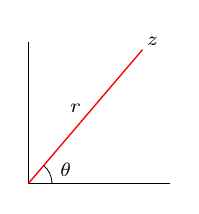
\begin{tikzpicture}[scale=.5]
  \draw[line width=.3pt] (0,3.6)--(0,0)--(3.6,0);
  \draw[red,line width=.5pt] (0,0)--node[above left=-2pt,font=\scriptsize,black]{$r$}
    (2.9,3.4) node[above right=-2pt,font=\scriptsize,black]{$z$};
  \draw[line width=.3pt] (.6,0) arc (0:49.5:.6);
  \node[font=\scriptsize] at (.95,.35) {$\theta$};
\end{tikzpicture}}{Representation of a complex number with polar coordinates.}%
For the proof below, we need to know that every $z\in\C$ has a square root in
$\C$. To show this, write
\[ z = r(\cos\theta + i\sin\theta), \]
where $r$ is the length of the line segment in the complex plane from the origin
to $z$ and $\theta$ is the angle of that line segment with the positive
horizontal axis. Then
\[ \sqrt{r}\Bigl(\cos\tfrac{\theta}{2} + i\sin\tfrac{\theta}{2}\Bigr) \]
is a square root of $z$, as you can verify by showing that the square of the
complex number above equals $z$.

\begin{result}[Over $\C$, invertible operators have square roots]\label{ax:8.41}
Suppose $V$ is a complex vector space and $T\in\Lin(V)$ is invertible. Then $T$
has a square root.
\end{result}

\begin{proof}
Let $\lambda_1,\dots,\lambda_m$ be the distinct eigenvalues of $T$. For each
$k$, there exists a nilpotent operator $T_k\in\Lin\bigl(G(\lambda_k,T)\bigr)$
such that $T|_{G(\lambda_k,T)}=\lambda_kI+T_k$ [see \ref{ax:8.22}(b)]. Because
$T$ is invertible, none of the $\lambda_k$'s equals $0$, so we can write
\[ T|_{G(\lambda_k,T)} = \lambda_k\Bigl(I+\frac{T_k}{\lambda_k}\Bigr) \]
for each $k$. Because $T_k/\lambda_k$ is nilpotent, $I+T_k/\lambda_k$ has a
square root (by \ref{ax:8.39}). Multiplying a square root of the complex number
$\lambda_k$ by a square root of $I+T_k/\lambda_k$, we obtain a square root
$R_k$ of $T|_{G(\lambda_k,T)}$.

By the generalized eigenspace decomposition (\ref{ax:8.22}), a typical vector
$v\in V$ can be written uniquely in the form
\[ v = u_1+\cdots+u_m, \]
where each $u_k$ is in $G(\lambda_k,T)$. Using this decomposition, define an
operator $R\in\Lin(V)$ by
\[ Rv = R_1u_1+\cdots+R_mu_m. \]
You should verify that this operator $R$ is a square root of $T$, completing the
proof.
\end{proof}

By imitating the techniques in this subsection, you should be able to prove that
if $V$ is a complex vector space and $T\in\Lin(V)$ is invertible, then $T$ has a
$k^{\text{th}}$ root for every positive integer $k$.

\subsection{Jordan Form}

We know that if $V$ is a complex vector space, then for every $T\in\Lin(V)$
there is a basis of $V$ with respect to which $T$ has a nice upper-triangular
matrix (see \ref{ax:8.37}). In this subsection we will see that we can do even
better---there is a basis of $V$ with respect to which the matrix of $T$
contains $0$'s everywhere except possibly on the diagonal and the line directly
above the diagonal.

We begin by looking at two examples of nilpotent operators.

\begin{example}[Nilpotent operator with nice matrix]\label{ax:8.42}
Let $T$ be the operator on $\C^4$ defined by
\[ T(z_1,z_2,z_3,z_4) = (0,z_1,z_2,z_3). \]
Then $T^4=0$; thus $T$ is nilpotent. If $v=(1,0,0,0)$, then $T^3v,T^2v,Tv,v$ is
a basis of $\C^4$. The matrix of $T$ with respect to this basis is
\[ \begin{pmatrix}
0&1&0&0\\
0&0&1&0\\
0&0&0&1\\
0&0&0&0
\end{pmatrix}. \]
\end{example}

The next example of a nilpotent operator has more complicated behavior than the
example above.

\begin{example}[Nilpotent operator with slightly more complicated matrix]\label{ax:8.43}
Let $T$ be the operator on $\C^6$ defined by
\[ T(z_1,z_2,z_3,z_4,z_5,z_6) = (0,z_1,z_2,0,z_4,0). \]
Then $T^3=0$; thus $T$ is nilpotent. In contrast to the nice behavior of the
nilpotent operator of the previous example, for this nilpotent operator there
does not exist a vector $v\in\C^6$ such that $T^5v,T^4v,T^3v,T^2v,Tv,v$ is a
basis of $\C^6$. However, if we take $v_1=(1,0,0,0,0,0)$, $v_2=(0,0,0,1,0,0)$,
and $v_3=(0,0,0,0,0,1)$, then $T^2v_1,Tv_1,v_1,Tv_2,v_2,v_3$ is a basis of
$\C^6$. The matrix of $T$ with respect to this basis is
\[ \begin{pmatrix}
\begin{pmatrix}0&1&0\\0&0&1\\0&0&0\end{pmatrix}
  & \begin{matrix}0&0\\0&0\\0&0\end{matrix}
  & \begin{matrix}0\\0\\0\end{matrix}\\
\begin{matrix}0&0&0\\0&0&0\end{matrix}
  & \begin{pmatrix}0&1\\0&0\end{pmatrix}
  & \begin{matrix}0\\0\end{matrix}\\
\begin{matrix}0&0&0\end{matrix}
  & \begin{matrix}0&0\end{matrix}
  & \begin{pmatrix}0\end{pmatrix}
\end{pmatrix}. \]
Here the inner matrices are blocked off to show that we can think of the
6-by-6 matrix above as a block diagonal matrix consisting of a 3-by-3 block
with $1$'s on the line above the diagonal and $0$'s elsewhere, a 2-by-2 block
with $1$ above the diagonal and $0$'s elsewhere, and a 1-by-1 block
containing~$0$.
\end{example}

Our next goal is to show that every nilpotent operator $T\in\Lin(V)$ behaves
similarly to the operator in the previous example. Specifically, there is a
finite collection of vectors $v_1,\dots,v_n\in V$ such that there is a basis of
$V$ consisting of the vectors of the form $T^jv_k$, as $k$ varies from $1$ to
$n$ and $j$ varies (in reverse order) from $0$ to the largest nonnegative
integer $m_k$ such that $T^{m_k}v_k\ne0$. With respect to this basis, the matrix
of $T$ looks like the matrix in the previous example. More specifically, $T$
has a block diagonal matrix with respect to this basis, with each block a
square matrix that is $0$ everywhere except on the line above the diagonal.

In the next definition, the diagonal of each $A_k$ is filled with some
eigenvalue $\lambda_k$ of $T$, the line directly above the diagonal of $A_k$ is
filled with $1$'s, and all other entries in $A_k$ are $0$ (to understand why
each $\lambda_k$ is an eigenvalue of $T$, see \ref{ax:5.41}). The
$\lambda_k$'s need not be distinct. Also, $A_k$ may be a 1-by-1 matrix
$(\lambda_k)$ containing just an eigenvalue of $T$. If each $\lambda_k$ is $0$,
then the next definition captures the behavior described in the paragraph above
(recall that if $T$ is nilpotent, then $0$ is the only eigenvalue of $T$).

\begin{definition}[Jordan basis]\label{ax:8.44}
Suppose $T\in\Lin(V)$. A basis of $V$ is called a \emph{Jordan basis} for $T$
if with respect to this basis $T$ has a block diagonal matrix
\[ \begin{pmatrix}
A_1 & & 0\\
& \ddots & \\
0 & & A_p
\end{pmatrix} \]
in which each $A_k$ is an upper-triangular matrix of the form
\[ A_k = \begin{pmatrix}
\lambda_k & 1 & & 0\\
& \ddots & \ddots & \\
& & \ddots & 1\\
0 & & & \lambda_k
\end{pmatrix}. \]
\end{definition}

Most of the work in proving that every operator on a finite-dimensional complex
vector space has a Jordan basis occurs in proving the special case below of
nilpotent operators. This special case holds on real vector spaces as well as
complex vector spaces.

\begin{result}[Every nilpotent operator has a Jordan basis]\label{ax:8.45}
Suppose $T\in\Lin(V)$ is nilpotent. Then there is a basis of $V$ that is a
Jordan basis for $T$.
\end{result}

\begin{proof}
We will prove this result by induction on $\dim V$. To get started, note that
the desired result holds if $\dim V=1$ (because in that case, the only nilpotent
operator is the $0$ operator). Now assume that $\dim V>1$ and that the desired
result holds on all vector spaces of smaller dimension.

Let $m$ be the smallest positive integer such that $T^m=0$. Thus there exists
$u\in V$ such that $T^{m-1}u\ne0$. Let
\[ U = \spn(u,Tu,\dots,T^{m-1}u). \]
The list $u,Tu,\dots,T^{m-1}u$ is linearly independent (see Exercise~2 in
Section~8A). If $U=V$, then writing this list in reverse order gives a Jordan
basis for $T$ and we are done. Thus we can assume that $U\ne V$.

Note that $U$ is invariant under $T$. By our induction hypothesis, there is a
basis of $U$ that is a Jordan basis for $T|_U$. The strategy of our proof is
that we will find a subspace $W$ of $V$ such that $W$ is also invariant under
$T$ and $V=U\oplus W$. Again by our induction hypothesis, there will be a basis
of $W$ that is a Jordan basis for $T|_W$. Putting together the Jordan bases for
$T|_U$ and $T|_W$, we will have a Jordan basis for $T$.

Let $\varphi\in V'$ be such that $\varphi(T^{m-1}u)\ne0$. Let
\[ W = \bigl\{v\in V : \varphi(T^kv)=0 \text{ for each } k=0,\dots,m-1\bigr\}. \]
Then $W$ is a subspace of $V$ that is invariant under $T$ $\bigl($the invariance
holds because if $v\in W$ then $\varphi\bigl(T^k(Tv)\bigr)=0$ for
$k=0,\dots,m-1$, where the case $k=m-1$ holds because $T^m=0\bigr)$. We will
show that $V=U\oplus W$, which by the previous paragraph will complete the
proof.

To show that $U+W$ is a direct sum, suppose $v\in U\cap W$ with $v\ne0$.
Because $v\in U$, there exist $c_0,\dots,c_{m-1}\in\F$ such that
\[ v = c_0u + c_1Tu + \cdots + c_{m-1}T^{m-1}u. \]
Let $j$ be the smallest index such that $c_j\ne0$. Apply $T^{m-j-1}$ to both
sides of the equation above, getting
\[ T^{m-j-1}v = c_jT^{m-1}u, \]
where we have used the equation $T^m=0$. Now apply $\varphi$ to both sides of
the equation above, getting
\[ \varphi(T^{m-j-1}v) = c_j\varphi(T^{m-1}u) \ne 0. \]
The equation above shows that $v\notin W$. Hence we have proved that
$U\cap W=\{0\}$, which implies that $U+W$ is a direct sum (see
\ref{ax:1.46}).

To show that $U\oplus W=V$, define $S\colon V\to\F^m$ by
\[ Sv = \bigl(\varphi(v),\varphi(Tv),\dots,\varphi(T^{m-1}v)\bigr). \]
Thus $\nul S=W$. Hence
\[ \dim W = \dim\nul S = \dim V - \dim\range S \ge \dim V - m, \]
where the second equality comes from the fundamental theorem of linear maps
(\ref{ax:3.21}). Using the inequality above, we have
\[ \dim(U\oplus W) = \dim U + \dim W \ge m + (\dim V - m) = \dim V. \]
Thus $U\oplus W=V$ (by \ref{ax:2.39}), completing the proof.
\end{proof}

\marginnote{Camille Jordan (1838--1922) published a proof of \ref{ax:8.46} in
1870.}%
Now the generalized eigenspace decomposition allows us to extend the previous
result to operators that may not be nilpotent. Doing this requires that we deal
with complex vector spaces.

\begin{result}[Jordan form]\label{ax:8.46}
Suppose $\F=\C$ and $T\in\Lin(V)$. Then there is a basis of $V$ that is a
Jordan basis for $T$.
\end{result}

\begin{proof}
Let $\lambda_1,\dots,\lambda_m$ be the distinct eigenvalues of $T$. The
generalized eigenspace decomposition states that
\[ V = G(\lambda_1,T)\oplus\cdots\oplus G(\lambda_m,T), \]
where each $(T-\lambda_kI)|_{G(\lambda_k,T)}$ is nilpotent (see
\ref{ax:8.22}). Thus \ref{ax:8.45} implies that some basis of each
$G(\lambda_k,T)$ is a Jordan basis for $(T-\lambda_kI)|_{G(\lambda_k,T)}$. Put
these bases together to get a basis of $V$ that is a Jordan basis for $T$.
\end{proof}

% ------------------------------------------------------------------ exercises
\begin{exc}

\begin{exercise}
Suppose $T\in\Lin(\C^3)$ is the operator defined by
$T(z_1,z_2,z_3)=(z_2,z_3,0)$. Prove that $T$ does not have a square root.
\end{exercise}

\begin{exercise}
Define $T\in\Lin(\F^5)$ by
$T(x_1,x_2,x_3,x_4,x_5)=(2x_2,3x_3,-x_4,4x_5,0)$.
\begin{parts}
\item Show that $T$ is nilpotent.
\item Find a square root of $I+T$.
\end{parts}
\end{exercise}

\begin{exercise}
Suppose $V$ is a complex vector space. Prove that every invertible operator on
$V$ has a cube root.
\end{exercise}

\begin{exercise}
Suppose $V$ is a real vector space. Prove that the operator $-I$ on $V$ has a
square root if and only if $\dim V$ is an even number.
\end{exercise}

\begin{exercise}
Suppose $T\in\Lin(\C^2)$ is the operator defined by $T(w,z)=(-w-z,9w+5z)$.
Find a Jordan basis for $T$.
\end{exercise}

\begin{exercise}
Find a basis of $\Poly_4(\R)$ that is a Jordan basis for the differentiation
operator $D$ on $\Poly_4(\R)$ defined by $Dp=p'$.
\end{exercise}

\begin{exercise}
Suppose $T\in\Lin(V)$ is nilpotent and $v_1,\dots,v_n$ is a Jordan basis for
$T$. Prove that the minimal polynomial of $T$ is $z^{m+1}$, where $m$ is the
length of the longest consecutive string of $1$'s that appears on the line
directly above the diagonal in the matrix of $T$ with respect to
$v_1,\dots,v_n$.
\end{exercise}

\begin{exercise}
Suppose $T\in\Lin(V)$ and $v_1,\dots,v_n$ is a basis of $V$ that is a Jordan
basis for $T$. Describe the matrix of $T^2$ with respect to this basis.
\end{exercise}

\begin{exercise}
Suppose $T\in\Lin(V)$ is nilpotent. Explain why there exist
$v_1,\dots,v_n\in V$ and nonnegative integers $m_1,\dots,m_n$ such that (a)
and (b) below both hold.
\begin{parts}
\item $T^{m_1}v_1,\dots,Tv_1,v_1,\dots,T^{m_n}v_n,\dots,Tv_n,v_n$ is a basis
  of $V$.
\item $T^{m_1+1}v_1=\cdots=T^{m_n+1}v_n=0$.
\end{parts}
\end{exercise}

\begin{exercise}
Suppose $T\in\Lin(V)$ and $v_1,\dots,v_n$ is a basis of $V$ that is a Jordan
basis for $T$. Describe the matrix of $T$ with respect to the basis
$v_n,\dots,v_1$ obtained by reversing the order of the $v$'s.
\end{exercise}

\begin{exercise}
Suppose $T\in\Lin(V)$. Explain why every vector in each Jordan basis for $T$ is
a generalized eigenvector of $T$.
\end{exercise}

\begin{exercise}
Suppose $T\in\Lin(V)$ is diagonalizable. Show that $\Mat(T)$ is a diagonal
matrix with respect to every Jordan basis for $T$.
\end{exercise}

\begin{exercise}
Suppose $T\in\Lin(V)$ is nilpotent. Prove that if $v_1,\dots,v_n$ are vectors
in $V$ and $m_1,\dots,m_n$ are nonnegative integers such that
\[ T^{m_1}v_1,\dots,Tv_1,v_1,\dots,T^{m_n}v_n,\dots,Tv_n,v_n \text{ is a basis
of } V \]
and
\[ T^{m_1+1}v_1=\cdots=T^{m_n+1}v_n=0, \]
then $T^{m_1}v_1,\dots,T^{m_n}v_n$ is a basis of $\nul T$.
\exnote{This exercise shows that $n=\dim\nul T$. Thus the positive integer $n$
that appears above depends only on $T$ and not on the specific Jordan basis
chosen for $T$.}
\end{exercise}

\begin{exercise}
Suppose $\F=\C$ and $T\in\Lin(V)$. Prove that there does not exist a direct sum
decomposition of $V$ into two nonzero subspaces invariant under $T$ if and only
if the minimal polynomial of $T$ is of the form $(z-\lambda)^{\dim V}$ for some
$\lambda\in\C$.
\end{exercise}
\end{exc}
